\section{rSLA implementation}\label{runtime} \todomohamed{rSLA implementation}

rSLA is implemented as a DSL for cloud SLAs and the engine that supports their overall management aspects. As shown in Figure~\ref{fig:runtime}, rSLA engine provides support for 
the following loosely coupled SLA management operations:
\begin{enumerate}
\item SLA creation and activation,
\item monitoring and measurement of service metrics as specified in the SLA,
\item storage and processing of observed service metric values and of SLO evaluation results,
\item scheduling of rSLA objects to collect observations and evaluate SLOs according to their 
specified schedules
\item service level evaluation 
\item notifications and reporting
\end{enumerate}

The next paragraphs highlight rSLA implementation aspects for all supported operations.

\subsection{SLA creation and activation}

As discussed in Section~\ref{dsl}, rSLA editing takes place using ruby programming blocks. The rSLA language takes advantage of this Ruby coding feature and exposes rSLA objects 
through blocks that respect our DSL. When an rSLA runtime engine reads a new rSLA block, it generates a new rSLA object that belongs to the block related class. The 
attributes and function behavior of the generated object are mapped from the ruby block context using the DSL. 

Listing \ref{basescript} describes an rSLA sample for the creation of an SLA and a base metric. This SLA could be submitted to an rSLA service runtime to generate the 
two respective objects. Then we could activate the SLA by triggering a schedule for the value measurement of the base metric.

\begin{minipage}{0.9\textwidth}
\begin{lstlisting}[language=Ruby, basicstyle=\small\normalfont\sffamily, breaklines=true,  captionpos=b, mathescape=true, caption=rSLA SLA (lines 1-4) and basemetric (lines 6-19) 
creation script, label=basescript, numbers=left, numbersep=5pt, numberstyle=\tiny] 
sla do
  tenant "Demo"
  provider "IBM"
end  

basemetric do
    name "bareMetalProvisioning"
    unit "provisioningtime"
    measurementdirective do
    	entity "baremetal"
    	type "jsonArray"
    	source "http://provisioningxlet.stage1.mybluemix.net/server/baremetal/provisioningtime" 
  	end
  schedule do    
  	frequency "1"
    unit "m"
    method "every"
  end
end
\end{lstlisting}
\end{minipage} 

Based on the SLA file, rSLA engine creates the needed objects (i.e., SLA and BaseMetric objects in this example). The engine interprets the file to fill the attributes of these 
objects. In the \emph{basemetric} block, the DSL user can define BaseMetric object attributes like the base metric name and measurement unit. Additionally, he can specify 
directives for the measurement of the created metric. A measurement directive represents a concept that is inherited from the WSLA specification \cite{wsla}. 

In rSLA DSL, a measurement directive is a block of statements that describes how to measure the value of the parent base metric. A measurement directive indicates also the 
result type that is expected from a base metric measurement. In the measurement directive block, the term entity is used for the representation of restful \footnote{REST: 
\url{http://en.wikipedia.org/wiki/Representational_state_transfer}} endpoints. A measurement directive object uses an attribute named $source$ to denote the restful endpoint for 
fetching the base metric value. %The rSLA MeasurementDirective class provides an example on how to define measurement directive objects for rSLA base metrics. Such example, 
%like the illustrated block of Listing \ref{basescript} can be extended accordingly. 

Last but not least, the DSL user can specify the details of a schedule for the measurement of the base metric. The schedule block details are explained in Section \ref{schedule}.

\subsection{Monitoring and measurement}
Any SLA management framework requires a tool for monitoring and measuring metric values. For monitoring, rSLA engine currently uses light weight mechanism 
called Xlets to handle the monitoring of base metric values. Section~\ref{deployment} describes in detail the Xlets and their usage along with the 
deployment of rSLA as a compliance service in a cloud environment.

In rSLA service, the collection of monitoring observations are controlled by one or more schedules. Every base metric follows its own schedule. Afterwards, the measured metric 
observations are collected to a backend database for further processing. 
\subsection{Storage and processing}
Currently, rSLA is deployed as a service on the IBM Bluemix platform \cite{bluemix} and is configured to use a Cloudant \cite{cloudant} database. Cloudant is a NoSQL database 
service provided by the PaaS. Based on the specified schedule, the values of base metrics are collected and stored as observation documents with a timestamp reflecting the 
measurement time and the associated base metric id. Cloudant uses map and reduce statements to collect and to efficiently process data values. 

The stored observations are required for the computation of composite metrics. Composite metrics eventually specify the aggregation expressions needed to calculate their values. 
And these latter are used for the service level evaluation. 

The persistence layer of rSLA is based on CouchRest \cite{couchrest} to map ruby objects to Cloudant documents. CouchRest  uses REST HTTP requests to map rSLA object properties in 
the database. Associations between rSLA objects are described through the rSLA Cloudant data schema. Figure \ref{schema} illustrates  associations between rSLA objects in a 
Cloudant database.

Base, composite metrics as well as SLOs are associated with an SLA instance by a \textit{belongs to} relationship. Similarly, observations \textit{belongs to} a base 
metric and evaluations and notifications data to an SLO. 

The \textit{belongs to} feature is defined in the CouchRest model as a property for the association of documents. It could be seen as an artificial foreign 
key to create associations between documents.  %It resembles a \textit{has-a} composition relationship 
%\footnote{\url{http://en.wikipedia.org/wiki/Has-a}} where a constituent object belongs to or is part of the definition of another object.

\begin{figure}
\centering
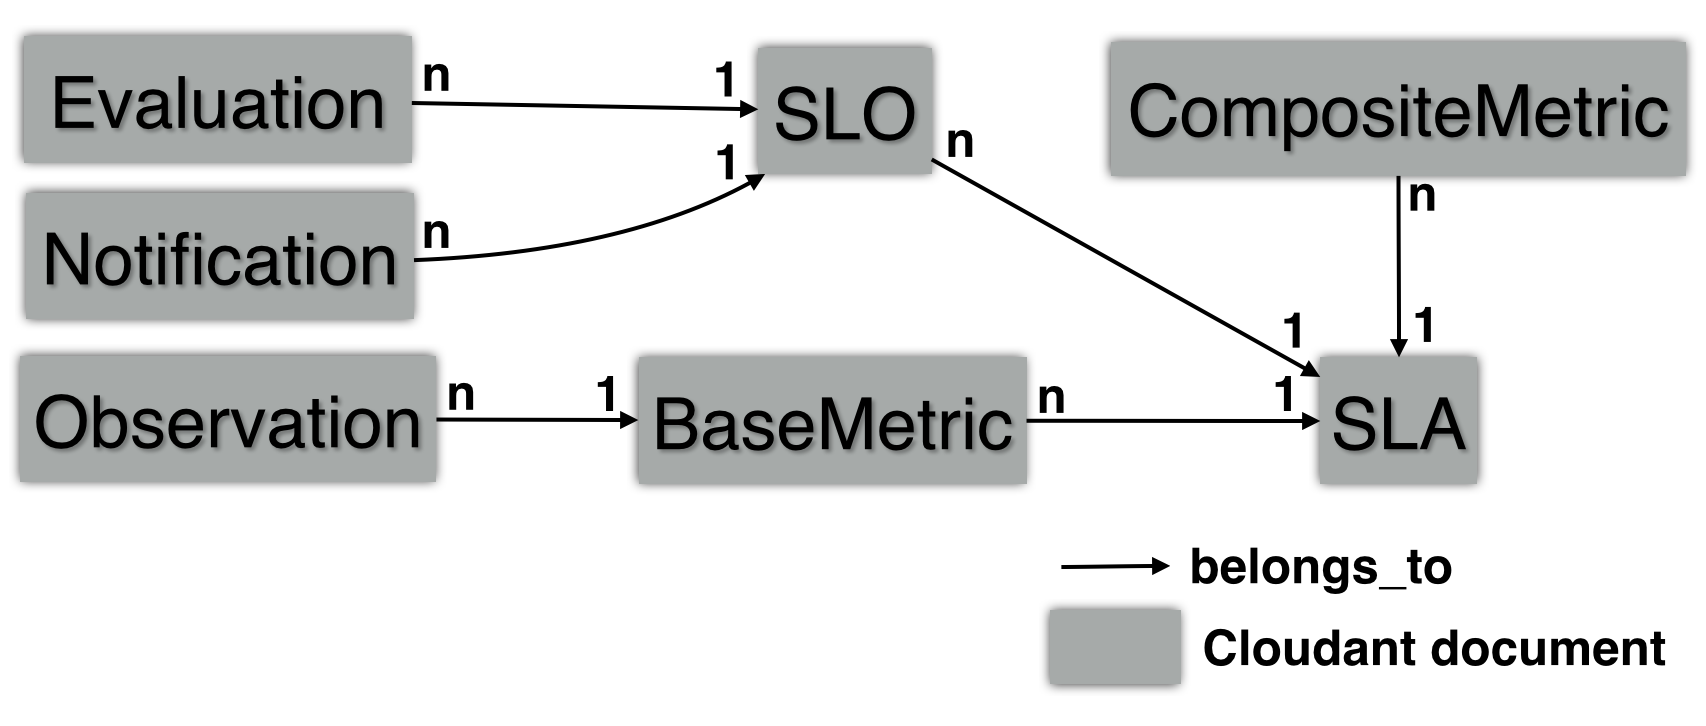
\includegraphics[width=0.8\textwidth]{pics/schema}
\caption{\label{schema} rSLA Cloudant object associations}
\end{figure}

Currently, processing of metric values may refer to compositions of base and/or composite metric values  for the creation of more aggregated 
composite metrics. %The definition of composite metrics represents the outcome from combining a set of base and/or composite metrics. 
The value computation of such metrics represents a computation that comprises values of other metrics. This computation is described in rSLA expressions.
As discussed in Section \ref{dsl}, expressions in rSLA denote free form statements that may take a conditional form or that may define data value computations. The computation for 
a composite metric value exemplifies an expression in rSLA. Composite metric values are used for the SLO evaluation. Expressions are used also for SLO evaluations as preconditions 
or objectives.

%Last but not least, the rSLA language library contains also a time series class that can be used for the application of statistical functions on time-series data sets. 

\subsection{Scheduling}\label{schedule}


When the rSLA engine receives a new SLA, it interprets this file to generate an SLA object in an \emph{INACTIVE} state. The inactive state indicates that 
the data collection of base metrics and the evaluation of SLOs are not yet associated to a scheduler. On SLA activation, the rSLA engine activates all base metrics and SLOs 
evaluation by sending their schedule description and id to the Scheduler. The Scheduler associates a job for each of the base metrics according to the specified scheduling data 
in the agreement. For the specified frequency, the Scheduler triggers a REST query to activate the data collection for base metrics or evaluations for SLOs. 

In rSLA, composite metrics do not include a schedule because the computation of their values depends from SLO evaluation events. The SLO definition specifies a schedule for the 
evaluation of precondition and objective expressions. Moreover, a scheduler orchestrates notification processes that send evaluation reports on scheduled intervals.

The orchestration of scheduling events represents a topic of on-going work. Currently, rSLA uses the open source Rufus-scheduler that is an in-memory Ruby scheduler. We endowed 
this Scheduler with REST interfaces in order to allow decoupling it from the other parts of rSLA engine. These REST interfaces allow creating and deleting different types of 
recurrent jobs for base metrics and for SLOs. 

\subsection{Service level evaluation and reporting}

Service level evaluation takes place at scheduled intervals. The frequency of service level evaluation is determined by the schedule attributes in 
the SLO definition. As discussed in Section \ref{dsl}, the definition of a service level objective encloses the description of a precondition and an objective expressions. These 
two expressions that follow sequential logic, define the evaluation conditions that designate if the state of an SLO is healthy or not. These expressions use composite and base 
metrics to evaluate the SLO.

Actually, service level evaluation is accompanied with a reporting step. This step consists on generating a notification based on the results of the evaluation. This notification 
contains eventually the list of violations that occurred and the percentage of the respect to the SLOs. Afterwards, this notification is sent to a reporting Xlet. This latter is 
endowed with a list of formatters that take as input a JSON document and generate a more readable format (e.g., CSV). The generated document is sent to the client to report the 
status of his provisioned resources. The reporting Xlet implements many protocols for reporting. Currently, we are using emails to send the reports to the clients. 